\documentclass{article}
\usepackage[en]{homework}
\usepackage{tensor}

\config{Physics\,-\,0}{2026 Spring}{3}

\begin{document}

\begin{problem}
	(30 pts) Consider a car moving on a circular road of radius $R$ that is
	inclined at an angle $\beta$. The coefficient of static friction is denoted by
	$\mu$.

    \begin{center}
        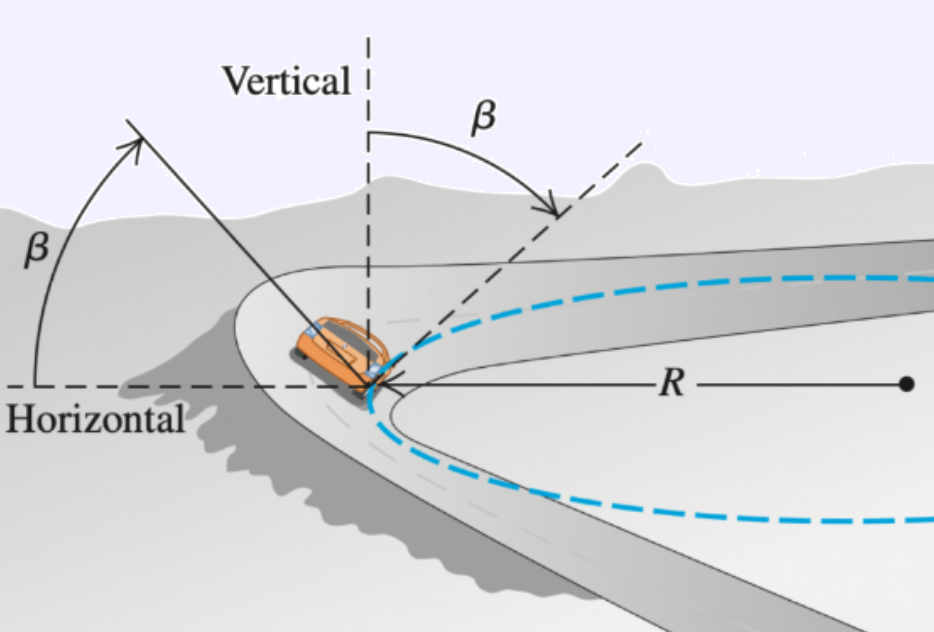
\includegraphics[width=0.4\textwidth]{PB1.png}
    \end{center}

	\begin{enumerate}[label=(\alph*)]
		\item (10 pts) Draw a diagram indicating the forces acting on
		the car and the direction of the acceleration.

		\item (10 pts) Find the maximum speed the car can be driven
		without sliding.

		\item (10 pts) Consider the maximum speed in two limits:
		(i) a frictionless road with arbitrary $\beta$ and (ii) a flat road with
		friction $\mu$. What is the value of $\beta$ in (i) necessary to reproduce
		the maximum speed in (ii)?
	\end{enumerate}
\end{problem}

\begin{solution}
    (a) The forces acting on the car and the direction of the acceleration are shown below:
    \begin{center}
        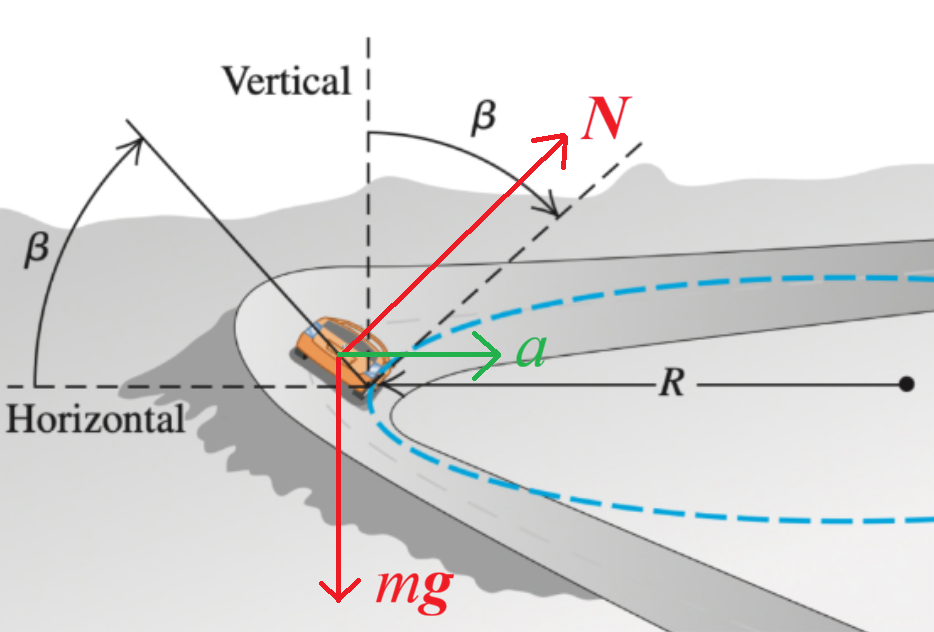
\includegraphics[width=0.4\textwidth]{SOL1.png}
    \end{center}
    There might be a frictional force \( f \) acting on the car, which is perpendicular to  \( \bo{N} \) and points towards or backwards the center, and therefore not shown in the figure.\par
    (b) Suppose the car is moving at the speed \( v \) , and the fricitional force is \( f \) , where the positive \( f \) represents pointing towards the center. Then by the Newton's Second Law, we get
    \[ \begin{cases}
        N \cos\beta-mg-f\sin\beta=0,\\
        N \sin\beta+f\cos\beta=mv^2/R,\\
        \abs{f}\leq \mu N.
    \end{cases} \] \par
    By solving the above equations, we can get the answers below:
    \begin{enumerate}[label=(\roman*)]
        \item  \( \mu<\cot\beta \) . Then 
        \[ N\le\frac{mg}{\cos\beta-\mu\sin\beta},\quad v\le\sqrt{Rg\,\frac{\sin\beta-\mu\cos\beta}{\cos\beta-\mu\sin\beta}}. \]
        \item \( \mu\geq\cot\beta \) . Then the car can be driven at any speed without sliding, and the maximum speed is infinite. 
    \end{enumerate}\par
    (c) In the limit of a frictionless road, the maximum speed is \( v=\sqrt{Rg\tan\beta} \). In the limit of a flat road with friction, the maximum speed is \( v=\sqrt{\mu Rg} \). Therefore, we can get
    \[ \tan\beta=\mu. \]
\end{solution}

\begin{problem}
    (20 pts) Ues the Levi-Civita symbol to prove the following properties of the cross product.
    \begin{enumerate}[label=(\alph*)]
        \item (10 pts) Scalar triple product identity:
        \[ \bo{A}\cdot(\bo{B}\times\bo{C})=\bo{B}\cdot(\bo{C}\times\bo{A})=\bo{C}\cdot(\bo{A}\times\bo{B}). \] 
        \item (10 pts) Vector triple product identity:
        \[ \bo{A}\times(\bo{B}\times\bo{C})=(\bo{A}\cdot\bo{C})\bo{B}-(\bo{A}\cdot\bo{B})\bo{C}. \]
    \end{enumerate}
\end{problem}

\begin{proof}
    Denote the components of \( \bo{A},\bo{B},\bo{C} \) as \( A^i,B^i,C^i \) respectively. We will use the Einstein summation convention into the proof. Note that there's no necessary to distinguish between upper and lower indices in this context, since we are working in a Cartesian coordinate system.\par
    (a) We have
    \[ \begin{aligned}
        \bo{A}\cdot(\bo{B}\times\bo{C}) &=A^i\epsilon_{ijk}B^jC^k,\\
        \bo{B}\cdot(\bo{C}\times\bo{A}) &=B^i\epsilon_{ijk}C^jA^k,\\
        \bo{C}\cdot(\bo{A}\times\bo{B}) &=C^i\epsilon_{ijk}A^jB^k.
    \end{aligned} \]
    Then the identity follows from the cyclic symmetry of the Levi-Civita symbol, i.e., \( \epsilon_{ijk}=\epsilon_{jki}=\epsilon_{kij} \).\par
    (b) We have
    \[ \begin{aligned}
        \bo{A}\times(\bo{B}\times\bo{C}) &=\epsilon\indices{^i_j^k}\bo{e}_iA^j\epsilon_{klm}B^lC^m
        =(\delta\indices{^i_{l}}\delta_{jm}-\delta\indices{^i_{m}}\delta_{jl})A^jB^lC^m\bo{e}_i\\
        &=A^jB^iC_j\bo{e}_i-A^jB_jC^i\bo{e}_i
        =(\bo{A}\cdot\bo{C})\bo{B}-(\bo{A}\cdot\bo{B})\bo{C}.
    \end{aligned} \]

\end{proof}

\begin{problem}
    (25 pts) A stick of length $L$ rests at an angle $\theta$ with respect to the
    ground, as illustrated below. A pivot is located at a position
    $x=\ell>L/2$ along the stick (here we take $x=0$ at the end on the ground).
    Find the magnitude of the force $\vec{F}$ along the vertical direction that
    needs to be applied to the raised end of the stick to make it start moving in
    the following cases.

    \begin{center}
        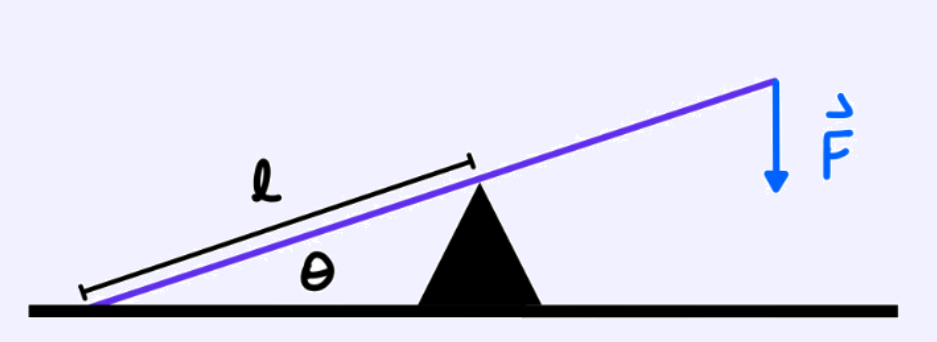
\includegraphics[width=0.4\textwidth]{PB3.png}
    \end{center}

    \begin{enumerate}[label=(\alph*)]
        \item (10 pts) When the stick has uniform mass $m$.

        \item (15 pts) When the stick has mass density given by
        \[
            \rho(x)=
            \begin{cases}
                \dfrac{2m}{L}, & 0\le x<\dfrac{L}{3},\\[4pt]
                \dfrac{m}{2L}, & \dfrac{L}{3}\le x<\dfrac{2L}{3},\\[4pt]
                \dfrac{m}{2L}, & \dfrac{2L}{3}\le x\le L.
            \end{cases}
        \]
    \end{enumerate}
\end{problem}

\begin{solution}
    Denote the coordinate of the center of mass of the stick as \( x_\mathrm{c} \) . by the torque equilibrium about the pivot, we can get
    \[ Mg(l-x_\mathrm{c})=F(L-l)\implies F=Mg\frac{l-x_\mathrm{c}}{L-l}, \] 
    where \( M \) is the total mass of the stick.\par
    (a) It's clear that \( x_\mathrm{c}=L/2 \) and \( M=m \) . Then 
    \[ F=mg\frac{2l-L}{2L-2l}. \] \par 
    (b) \( M \) and \( x_\mathrm{c} \) is given by
    \[ M=\int_{0}^{L} \rho(x)\d x=M,\quad x_\mathrm{c}=\frac{1}{M}\int_{0}^{L} x\rho(x)\d x=\frac{L}{3}. \] 
    Then 
    \[ F=mg\frac{3l-L}{3L-3l}. \] 

\end{solution}

\begin{problem}
    (25 pts) The wings of a plane are shaped in such a way that air flowing over
    the wings is pushed down and slightly forward, so from Newton's third law the
    air exerts a force back on the wings that is up and slightly backwards. The
    upward force is the lift force that keeps the plane in the air, while the
    backward force is called induced drag and is inversely proportional to $v^2$,
    where $v$ is the speed of the plane. If we also include air resistance, which
    is proportional to $v^2$, the total air resistance force experienced by the
    plane is
    \[
        F_{\mathrm{air}}=\alpha v^2+\frac{\beta}{v^2},
    \]
    where $\alpha$ and $\beta$ are parameters that depend on the plane and the
    density of the air.
    \begin{center}
        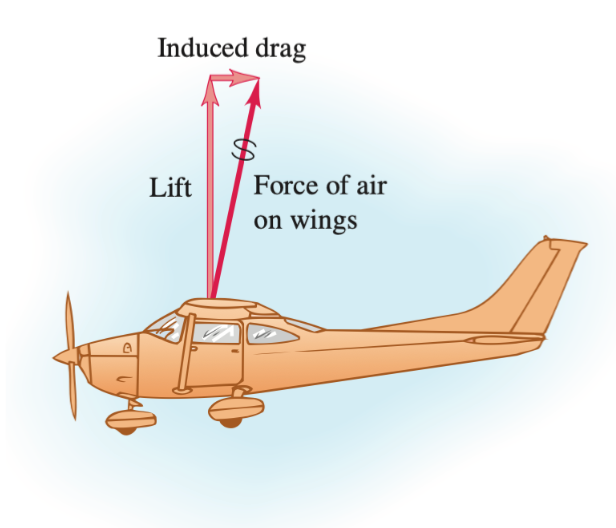
\includegraphics[width=0.4\textwidth]{PB4.png}
    \end{center}\par
    Assume that the plane flies at a constant speed, meaning that the forward
    force provided by the engine exactly balances air resistance, and that it
    performs a fixed amount of work (since the airplane has a finite amount of
    fuel) denoted by $W_0$.

    \begin{enumerate}[label=(\alph*)]
        \item (10 pts) Find the speed for which the plane has a maximum range (displacement).
        \item (10 pts) Find the speed for which the plane spends the longest time
        in the air.
        \item (5 pts) Compare the force due to air resistance $F_{\mathrm{air}}$
        in each case and determine which one is larger.
    \end{enumerate}
\end{problem}

\begin{solution}
    (a) The range of the plane is given by
    \[ R=\frac{W_0}{F_\mathrm{air}}=\frac{W_0}{\alpha v^2+\beta v^{-2}}. \] 
    To maximize \( R \) , we can minimize \( F_\mathrm{air} \) . By solving the equation \( \d F_\mathrm{air}/\d v=0 \) , we can get
    \[ v=\sqrt[4]{{\beta/\alpha}}. \] \par
    (b) The time spent in the air is given by
    \[ T=\frac{W_0}{\alpha v^3+\beta v^{-1}}. \]
    To maximize \( T \) , we can minimize \( \alpha v^3+\beta v^{-1} \) . By solving the equation \( \d(\alpha v^3+\beta v^{-1})/\d v=0 \) , we can get
    \[ v=\sqrt[4]{{\beta/3\alpha}}. \] \par
    (c) The force due to air resistance in (b) is larger.
\end{solution}





\end{document}